% !TeX encoding = UTF-8
% !TeX program = xelatex
\documentclass[12pt, a4paper]{article}
\usepackage{graphicx}
\usepackage{amsmath}
\usepackage{xeCJK} % 须放在\usepackage{}列中足够前的位置
\usepackage{fontspec}
\usepackage{caption}
\usepackage{enumerate}
\usepackage{setspace}
\usepackage{array} % 製作表格必須的宏包
\usepackage{tabularx} % 自動調整列寬的表格宏包
\usepackage{adjustbox}
\usepackage{geometry}
\setCJKfamilyfont{heiti}{Heiti TC}
\CJKfamily{heiti}
\setmainfont{Arial}
\setstretch{1.5}


\begin{document}
\begin{center}
  {\Huge 邏輯設計實驗} \\[2.5cm]
  {\Huge Lab8} \\[1.5cm]
  {\Huge 比較器與多工器} \\ [4.5cm]
  \hspace{.6in}
  \begin{minipage}[t]{.4\linewidth}
    {\Large 班級:資訊一甲}\\[0.5cm]
    {\Large 學號:D1109023}\\[0.5cm]
    {\Large 姓名:楊孟憲}
  \end{minipage}    
\end{center}

\newpage
%\fontsize{30pt}{36pt}\selectfont 
%\normalsize

\begin{description}
  \fontsize{22pt}{25pt}\selectfont 
    \item [一、]摘要 
      \begin{enumerate}
        \fontsize{20pt}{22pt}\selectfont
          \item 一位元關係比較器\\[.5cm]
            \begin{minipage}{\linewidth}
              \fontsize{16pt}{18pt}\selectfont
              比較 A 和 B,將兩值利用邏輯閘判斷其大小。
              其中輸出的G、E、L代表(Greater, Equal, Less) \\
              \normalsize
            \end{minipage}
            \begin{description}
              \fontsize{16pt}{20}\selectfont
                \item [(1)] 真值表 \\[.5cm]
                    \begin{tabular}{|c c|c c c|}
                      \hline
                      A & B & G & E & L \\
                      \hline
                      0 & 0 & 0 & 1 & 0 \\
                      \hline
                      0 & 1 & 0 & 0 & 1 \\
                      \hline
                      1 & 0 & 1 & 0 & 0 \\
                      \hline
                      1 & 1 & 0 & 1 & 0 \\
                      \hline
                    \end{tabular}\\

                \item [(2)] 函數 \\[.1cm]
                    $G = A\cdot \bar B$ \\ 
                    $E = A \cdot B + \bar A \cdot \bar B$ \\
                    $L = \bar A\cdot B$
                \newpage
                \item [(3)] 功能模組 \\[.4cm]
                  
\includegraphics[width=10cm]{./image/比較器.png} \\ [.5cm]
              \normalsize
            \end{description}
            \item 2 $\rightarrow$ 1 多工器\\
              \fontsize{16pt}{20pt}\selectfont
              \begin{samepage}              
                三個輸入 A, B, S,S 代表選擇器。
              \end{samepage}
              \begin{description}
                  \item [(1)] 選擇碼真值表
                    \begin{table}[h]
                      \centering
                      \label{tab:sample}
                      \begin{adjustbox}{width=.15\textwidth}
                      \begin{tabular}{ |c|c| }
                        \hline
                        S & Y \\
                        \hline
                        0 & B \\
                        \hline
                        1 & A \\
                        \hline
                      \end{tabular}
                      \end{adjustbox}
                      \end{table}
                  \item [(2)] 組合函示表示式\\ 
                      $Y = A\cdot S + B\cdot \bar S$
              \end{description}
              \normalsize
        \normalsize
      \end{enumerate}
    \item [二、]實驗結果
      \newpage
      \begin{description}
        \fontsize{20pt}{22pt}\selectfont
        \item [1.]實驗一
          \fontsize{16pt}{18pt}\selectfont
            \begin{description}
              \item [$\bullet$]用兩個四位元比較器7485及一般邏輯閘完成下列設計,當輸入小於4時,輸出a會亮,而當輸入小於等於10大於等於4時,輸出b會亮,當輸入大於10時,輸出c會亮。 \\[.2cm]
              
\includegraphics[width=10cm]{./image/ex1_p.png}
              \fontsize{18pt}{20pt}
              \item [(1)]實作邏輯 \\[.3cm]
                \begin{samepage}
                  \fontsize{16pt}{18pt}
                  利用兩個位元比較器來實作判斷輸入4 bit 介在哪個區間,即哪個燈應該亮。\\
                  $\bullet$第一個 $7485_{i}$ 來判斷輸入與 4 的關係,輸出即為 $G_{i}, E_{i}, L_{i}$\\
                  $\bullet$第二個 $7485_{k}$ 來判斷輸入與 10 的關係,輸出即為 $G_{k}, E_{k}, L_{k}$\\
                  定義好後再利用邏輯閘完成電路。\\
                  $\bullet$ 電路方程:\\
                  \bf$a = L_{i}$\\
                  $b = (G_{i} + E_{i})\cdot (L_{k} + E_{k})$\\
                  $c = G_{k}$
                  \normalfont
                \end{samepage}
              \item [(2)] 電路圖 \\[.5cm]
                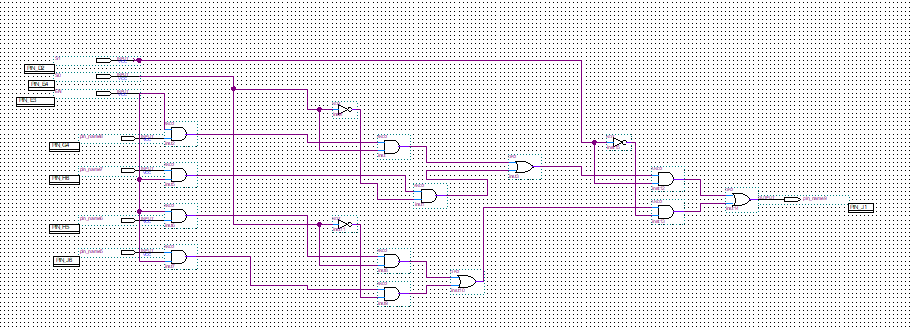
\includegraphics[width=13cm]{./image/ex1.png}          
            \end{description}
          \normalsize
          \fontsize{20pt}{22pt}\selectfont
        \item[2.] 實驗二 \\
              \fontsize{16pt}{18pt}\selectfont
                $\bullet$ 利用邏輯閘實現一個 2 $\rightarrow$ 1多工器。\\
                $\bullet$ 利用前面已設計的2 $\rightarrow$ 1多工器, 實現一個4 $\rightarrow$ 1多工器。
              \fontsize{18pt}{20pt}\selectfont
              \begin{description}
                \item[(1)] 實作邏輯\\
                  \fontsize{16pt}{18pt}
                  \begin{samepage}
                    我們有兩個bit的選擇訊號 $S_{0}, S_{1}$,我們可以觀察真值表得出電路函示。\\
                    \bf 真值表:
                    \begin{table}[h]
                      \centering
                      \begin{adjustbox}{width=.3\textwidth}
                        \begin{tabular}{ |c c|c| }
                          \hline
                          $S_{0}$ & $S_{1}$ & $Y$ \\
                          \hline
                          0 & 0 & A \\
                          \hline
                          0 & 1 & B \\
                          \hline
                          1 & 0 & C \\
                          \hline
                          1 & 1 & D \\
                          \hline
                        \end{tabular}
                      \end{adjustbox}
                    \end{table}\\
                      \bf 電路函示:\\
                      $Y = ((A\cdot S_{0} + B\cdot \bar{S_{0}})\cdot S_{1}) + ((C\cdot S_{0} + D\cdot \bar{S_{0}})\cdot \bar{S_{1}})\cdot EN$
                  \end{samepage}
                \fontsize{18pt}{20pt}
                \item[(2)] 電路圖 \\[.3cm]
                  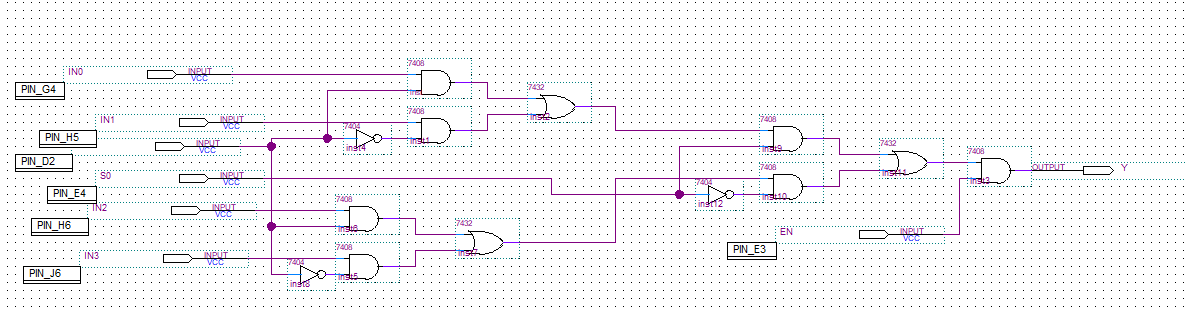
\includegraphics[width=15cm]{./image/ex2.png} \\[.3cm]
              \end{description}
        \fontsize{20pt}{22pt}\selectfont
        \item[3.] 實驗三 \\
            \fontsize{16pt}{18pt}\selectfont
            $\bullet$輸入今天的日期並用七段顯示器顯示。 \\
            X=0, 七段顯示器出現今天日期的十位數字\\
            X=1, 七段顯示器出現今天日期的個位數字
            \normalsize
            \begin{description}
              \fontsize{18pt}{20pt}\selectfont
              \item[(1)]實作邏輯 \\
                \begin{samepage}
                  \fontsize{16pt}{18pt}\selectfont
                    輸入為兩個 4 bits的數值,以及一個bit的x ,使用2 $\rightarrow$ 1 選擇器判斷 x 的狀態,在選擇輸出十位數字或是個位數字。
                  \normalsize
                \end{samepage}
              \fontsize{18pt}{20pt}\selectfont
              \item[(2)]電路圖 \\[.2cm] 
              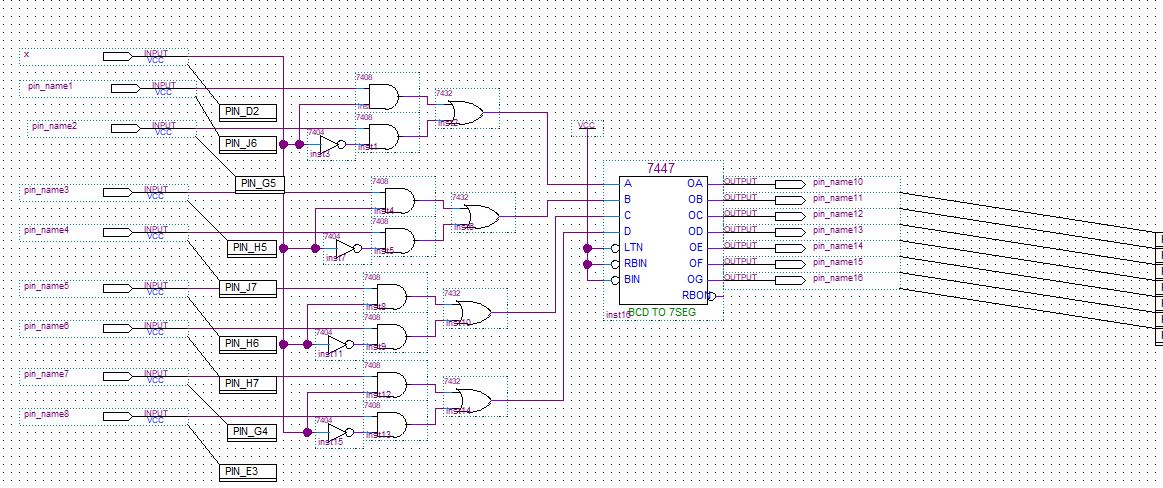
\includegraphics[width=13cm]{./image/ex3.png}
            \end{description}
        \normalsize
      \end{description}
    \item [三、]問題討論心得 \\[.6cm]
      \begin{minipage}[t]{\linewidth}
        \fontsize{16}{18}\selectfont
          這次實驗學習使用比較器和多工器,我覺得多工器這個技術雖然背後用的 ic 比較多,但是在設計電路的時候可以用比較直觀的方式實作電路,這種技術也可以運用在很多情況。
          之後的實驗應該會常常使用到多工器來實作邏輯。
        \normalsize  
      \end{minipage}
  \normalsize
\end{description}

\end{document}

